\chapter{Introduction}
% Goal : 5-10 page talk before the talk
% maybe not 10 pages, but providing a general overview of the paper is the goal here
\section{Overview}
A significant body of work in the field of mobile computing has aimed to
address the inherent resource poverty of mobile devices using cloud or cloudlet
offload \cite{satya1996,satya2009}. Mobile devices perpetually lag behind
static devices in computational ability because of their size and weight
constraints \cite{satya2014}. Increased computational ability, at the same
level of hardware efficiency, demands higher energy consumption. This requires
larger batteries to preserve operating time, thereby increasing weight and
size---which are undesirable for mobile devices.  This is especially true for
unmanned aerial vehicles (UAVs), or drones, which spend most of their energy on
flight.  Increased drone weight leads to an upwards spiral in weight as larger
rotors and more powerful motors are needed to achieve the same amount of lift.
This requires larger batteries which, in turn, may require a more reinforced
aircraft structure, and so on.

Cloudlet offload addresses these issues by allowing mobile devices to remotely
execute computationally expensive tasks on static infrastructure that does not
need to be light or small. This allows mobile devices to retain their low
weight and small size, but possess computational abilities way beyond what
would otherwise be possible.

SteelEagle, an autonomous drone system, follows this approach \cite{bala2024}.
Its main tenet is the use of commerical-off-the-shelf (COTS) drones, which are
readily available at low cost but typically have minimal to no on-board
computational resoures.  Utilizing cloudlet offload, SteelEagle enables COTS
drones to perform much more intelligent tasks than what they were designed for,
and exhibit autonomous capabilities typically only found in larger, more
expensive drones.  SteelEagle focuses on active vision tasks which require the
ability to perform live video analytics during flight to determine the next
course of action. SteelEagle drones relay their camera video stream over a
commercial cellular network to a nearby on-ground edge server, a cloudlet,
which runs a computationally expensive pipeline involving neural networks to
perform tasks such as object detection (\cref{fig:steeleagle-drone-arch}).  This processing of the raw drone
sensor streams allows obtaining higher level semantic information about the
drone's physical environment, such as the distance to obstacles that present
the danger of a collision. The drone can then be sent piloting commands to
react, such as instructions to actuate to avoid an impending collision.

\begin{figure}[htbp]
\centerline{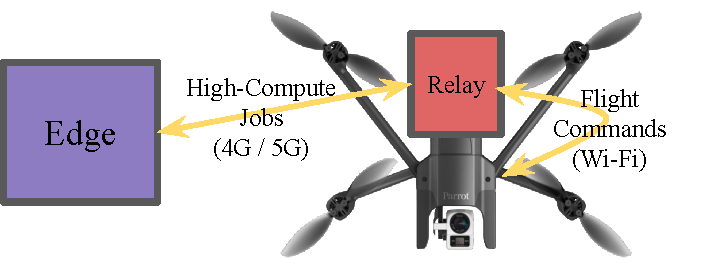
\includegraphics[width = .6\textwidth]{figs/steeleagle-drone-arch-cropped.pdf}}
\caption{Cloudlet Offload in SteelEagle}
\label{fig:steeleagle-drone-arch}
\end{figure}

An important consideration for SteelEagle is the agility of the resulting
system.  How quickly can a drone respond to a change in its environment? It is
the end-to-end latency of the entire execution pipeline, including sensing,
offloading, inferencing, decision making, and actuation, that defines the
agility. A high end-to-end latency can severely handicap the drone---it must
fly at a higher altitude or at lower speeds to be safe if it takes a long time
to identify obstacles and actuate to bypass them. Drone flight at a higher
altitude precludes close observation, and lower speeds make missions take
longer, limiting the capabilities of the drone. Search and rescue missions in
forests, and missions to aid policing operations in dense cities, for instance,
must fly at low altitudes while bypassing obstacles in the environment that
present a collision risk---trees branches, streetlight poles, utility
wires, and buildings---without impacting mission speed. Unless we can achieve
high agility, SteelEagle drones will struggle to perform these missions well.
Since these missions are one of the most compelling use cases for autonomous
drones, benchmarking the end-to-end pipeline to determine latency bottlenecks
and identifying opportunities for latency optimization is a very worthy pursuit.

The "Observe, Orient, Decide, Act" (OODA) loop framework devised by military
strategist John R. Boyd provides a framework to structure our investigation
into the end-to-end latency of SteelEagle. According to Boyd, decision-making
happens in a continuous iteration of these steps. Boyd attributed the faster
OODA loop of U.S. pilots flyng F-86s, because of the bubble-shaped canopy
offering better visibility and hydraulic controls that allowed for easier
switching between manoeuvres, as the reason the slower F-86s fared better than
the North Korean MiG-15s during the Korean War \cite{morton1995}. A system with
a tighter OODA loop corresponds to a more agile drone. Instead of measuring
just the overall system latency, performing a break down of the latency across
the OODA steps provides more insight into system latency bottlenecks. Ideally,
the decision stage, which involves inferencing, should be the slowest stage.

SteelEagle drones currently act as thin clients, performing no on-board
computation---they are controlled exclusively over the network. They transmit a
video stream from their camera to a cloudlet which determines the next course
of action based on an analysis of the received video, sent back to the drone
over the network. While this strategy allows treating consumer-grade
non-programmable drones as black boxes, it presents severe limitations. First,
SteelEagle drones struggle in areas with unreliable cell service and are
completely inoperable in regions without cellular coverage. Second, cloudlet
offload imposes an upper bound on drone agility as it adds the cost of a
round-trip latency to a cloudlet. As originally envisioned, cloudlets are
differentiated from clouds because of their physical proximity, which allows
application end-to-end response time to be just a few milliseconds. However, in
practice, the usage of commerical cellular networks for offload to the cloudlet
increases this latency to tens of milliseconds. In practice, this limits the
agility of the drone, as the reaction time is at least the round-trip time to
the cloudlet.

This thesis explores the use of onboard computation to mitigate these issues,
and the resulting impact on drone agility. In recent years, domain-specific
system-on-a-chip devices have become available that provide substantial
energy-efficient on-board computational resources through the inclusion of
hardware accelerators in the chip design. These chips can decode the video
stream generated by the drone and perform analytics using TensorFlow Lite
models, and often include 5G and Wi-Fi connectivity. Using such a chip as a
communications relay in SteelEagle allows us to continue treating the drone as
a black box, but employ new cloudlet offload tactics that result in tighter
OODA loops for use cases that can utilize the hardware accelerators, while
retaining the generality offered by cloudlet offload.

\section{Background: SteelEagle}

Autonomous drones perform tasks such as navigating between waypoints and
tracking moving objects without the need for a human pilot.  However,
autonomous drones today are large and expensive. Lightweight drones are more
appealing, as they present a smaller public safety hazard and thus face fewer
regulations. The FAA, for instance, has pre-authorized flights over people and
vehicles by drones weighing less than 250 g. On the other hand, cheaper drones
will help accelerate the uptake of autonomous drones in scenarios that stand to
benefit the most from their abilities. Search and rescue operations, as well as
wildlife conservation efforts that involve monitoring wildlife populations,
will benefit immensely from the abilities of drones to cover large areas
quickly. The potential for good increases exponentially with a swarm of drones
working cooperatively. Especially in rural areas with limited resources, for
instance, a swarm of drones working together could quickly scan large swathes
of land looking for an abducted child.

Over time, autonomous drones will
become cheaper and lighter as new ASIC designs are developed that are more
energy efficient and mass production lowers costs. Until then, leveraging edge
computing to add autonomous features to lighter consumer-grade drones at a much
lower price tag is a very appealing proposition. This is the software-hardware
co-evolution path that Satyanarayanan et al outlined, presenting offloading as
a way to "cheat" until ASIC designs are available \cite{satya21}.

Bala et al have demonstrated that even drones with a monocular camera can
perform tasks such as object tracking and depth inference reasonablly
well \cite{bala2024}. In their setup, Bala et al first attempted using a Samsung
Galaxy smartwatch as a communications relay, mounted on top of a Parrot Anafi
drone, for a total takeoff weight of about 360 g. The Samsung Galaxy smartwatch
is appealing because it is an enclosed system, including a battery and an
enclosure protected from the elements. It also has the ability to run Android
applications onboard.  However, the constant LTE tranmission on the watch
caused it to hit its thermal limits, which are set so that the watch can be
safely worn on the human wrist, and shut down.

As an alternative, Bala et al used the Onion Omega 2 system-on-a-chip device
\cite{onionomega2}. While the Omega 2 does not have the thermal limitations
present in the Galaxy smartwatch, it has very weak computational capabilities.
Intended for use as an IoT module, the Omega 2 runs the 580MHz MIPS 24KEc CPU
and has only 16 MB of flash storage. In the SteelEagle setup, a VPN tunnel
between the cloudlet and the Omega 2 over 4G LTE cellular allows communication
with the drone that is connected to the Omega 2 over Wi-Fi. The Omega 2's role
is to route packets between its Wi-Fi and LTE network interfaces, truly acting
as just a communications relay.

\section{Background: SteelEagle Benchmarks}
Bala et al performed experiments to measure the agility of the SteelEagle
system. The experiment setup involves setting up a stationary drone in a lab
setting, with its camera pointed at a display connected to the cloudlet, showing
the current timestamp in milliseconds. The drone camera captures images of this
timestamp and transmits them to the cloudlet through the SteelEagle pipeline.

\section{Motivation}


\section{Overview}


\section{Contributions}

The contributions of this thesis include
\begin{itemize}
  \item Things
\end{itemize}


\section{Organization}
